\documentclass[../main.tex]{subfiles}

\begin{document}
\begin{CJK*}{UTF8}{gbsn}

\section*{Exercice 1f}
On se demande si d'autres variables
dans le jeu de données pourraient être des facteurs confondants, et si l'on devrait stratifier le
test du Log-Rank sur l'une de ces variables. À partir de statistiques descriptives, de graphiques
et/ou d'arguments adaptés au contexte de l'étude, discuter de laquelle des variables du jeu de
données risque d'agir comme facteur confondant et reproduire le test du Log-Rank stratifié pour cette variable.
    
\paragraph{Solution}
Dans la vie quotidienne, on trouve que des personnes 
âgées ont plus grande probabilité de devenir aveugle. 
On soupçonne naturellement que l'âge
soit un facteur confondant qui influence la durée jusqu'à la cécité.
On analyse donc la variable \texttt{age}. 
Afin de confirmer cette intuition,
on classe les patients en deux groupes, \texttt{younger} et \texttt{older},
selon si l'âge du patient soit inférieur ou supérieur à l'âge médian
et trace les courbes de Kaplan-Meier pour ces deux groupes. 

\begin{lstlisting}
    median_age <- median(diabetic$age, na.rm = TRUE)
    diabetic$age_group <- ifelse(diabetic$age <= median_age, "younger", "older")
    result.kmage <- survfit(Surv(time, status) ~ age_group, data = diabetic)
    plot(result.kmage, main = 'Courbe de Kaplan-Meier', xlab = 'Temps en jours', ylab = 'Probabilite de survie', col = c("red", "blue"))
\end{lstlisting}

Le plot est :

\begin{figure}[H]
    \centering
    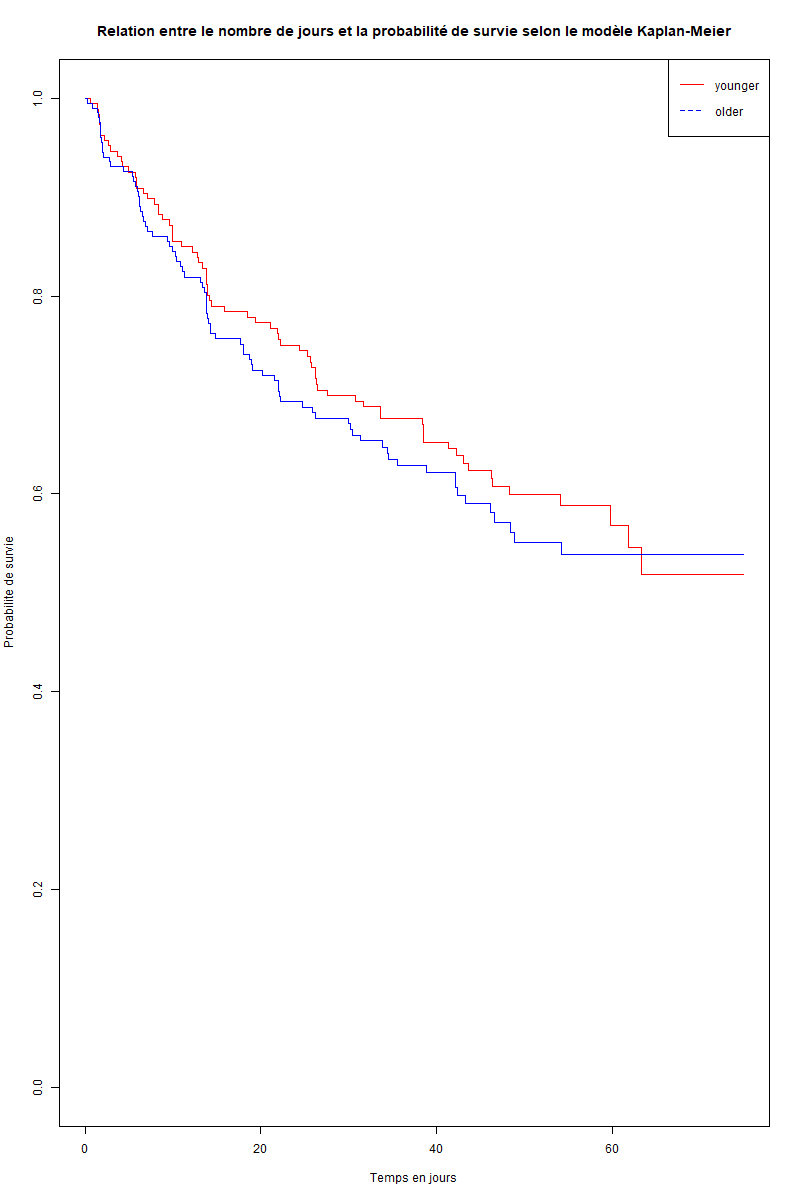
\includegraphics[width=0.4\textwidth]{1f.png}
    \label{fig:mesh1}
\end{figure}

Le graphique montre que la courbe \texttt{younger} est plus élevée que la courbe \texttt{older} 
à la plupart des moments.
On soupçonne que l'âge est à moins un bloc parce que 
la probabilité de survie soit plus 
élevée pour le groupe \texttt{younger} que pour le groupe \texttt{older}. 
Donc, on observe que le groupe \texttt{younger}
présente une probabilité de cécité plus faible que le groupe \texttt{older}.
Par conséquent, on conclut que l'âge est un facteur important.

On effectue le test de Log-Rank stratifié pour les deux groupes d'âge.

\begin{lstlisting}
    survdiff(Surv(time, status) ~ trt + strata(age), data = diabetic)
\end{lstlisting}

Le résultat est :

\begin{lstlisting}    
Call:
survdiff(formula = Surv(time, status) ~ trt + strata(age), data = diabetic)
        
        N Observed Expected (O-E)^2/E (O-E)^2/V
trt=0 197      101     71.9      11.8      23.4
trt=1 197       54     83.1      10.2      23.4
        
    Chisq= 23.4  on 1 degrees of freedom, p= 1e-06
\end{lstlisting}

Comme la p-valeur est $10^{-6}$,
il y a une différence significative dans le délai de cécité entre les deux groupes de traitement.
Même après stratification par âge, il existe encore une différence 
significative dans le risque de cécité entre le groupe \texttt{trt=1}
et le groupe de \texttt{trt=0}. 
On conclut que les patients du groupe de \texttt{trt=1} 
ont une probabilité de cécité plus faible que 
les patients du groupe \texttt{trt=0}. 

En conclusion, l'âge est un facteur important influençant la durée à la cécité 
et qu'il doit être pris en compte lors de l'élaboration des stratégies de traitement.
Dans tous les deux groupes d'âges, le traitement de laser diminue toujours 
le risque de cécité. ////

\end{CJK*}
\end{document}